 \documentclass[a4paper,11pt,twoside]{report}%pridat twoside, do [] pre obojstrannu tlac
    \pagestyle{headings}
    \usepackage[top=2.5cm, bottom=2.5cm, left=3.5cm, right=2cm]{geometry} %odporucane okraje

\usepackage[T1]{fontenc} %pekne makcene
\usepackage{amsmath}
\usepackage{mathtools}
\usepackage{amssymb}
\usepackage{graphicx}
\usepackage{graphics}
\usepackage{algorithmic}
\usepackage{algorithm}
\usepackage{listings}
%\usepackage{cite}

\graphicspath{ {pictures/} }
\renewcommand{\thesection}{\arabic{section}}

\author{Matus Behun}
\title{Cayley graphs of given diameter on linear groups}

\usepackage{hyperref}
    \hypersetup{colorlinks,citecolor=red,filecolor=black,linkcolor=blue,urlcolor=blue,pdftex}

\begin{document}
\setlength{\belowdisplayskip}{7pt} \setlength{\belowdisplayshortskip}{5pt}
\setlength{\abovedisplayskip}{7pt} \setlength{\abovedisplayshortskip}{5pt}

%====================================================================================================================================================
% FIRST PAGE
%====================================================================================================================================================
\begin{titlepage}
     \centering
     \begin{figure}[ht!]
     \centering
     \includegraphics[width=90mm]{logo.png}
     \end{figure}
     {\scshape\LARGE Slovak University of Technology in Bratislava \par}
     \vspace{1cm}
     {\scshape\Large Student scientific conference\par}
     \vspace{1.5cm}
     {\huge\bfseries Cayley graphs of given degree and diameter on linear groups\par}
     \vspace{2cm}
	 {\Large\itshape Mat�\v{s} Behun, 3.ro\v{c}n�k, MPM\par}
     \vfill
	 Supervisor\par
	 doc. RNDr. Jana \v{S}iagiov�, PhD. 
     \vfill
 
 % Bottom of the page
     {\large Bratislava 14th of April 2018}
 \end{titlepage}
 \newpage

%====================================================================================================================================================
% END OF FIRST PAGE
%====================================================================================================================================================

\section{Introduction}

In its simplest form, networks can be modeled by graphs in a natural way in which network nodes are represented by vertices of the graph and links between nodes are represented by undirected edges of the graph. Restrictions on the network, such as limits on the number of links attached to a node, or limits on the number of links needed to connect any two nodes, or the length of a shortest circuit, then transform to restrictions on the graph model (for the indicated cases these would be restrictions on vertex degrees, on the diameter, and on the girth of the graph).
\medskip

In graph theory this leads to two important problems: the {\em degree/diameter problem} to construct the largest possible graphs of a given maximum degree and a given diameter, and the {\em degree/girth problem} to construct the smallest possible regular graphs of a given degree and a given girth; in both cases the adjectives `large' and `small' refer to the order (i.e., the number of vertices) of a graph. The survey papers \cite{Mil-Sir} and \cite{Exo-Jaj}, respectively, contain a large amount of information on both problems. In this work we primarily address the degree/diameter problem restricted to Cayley graphs of certain two-dimensional linear groups, giving details in what follows.


\newpage

%====================================================================================================================================================
% INTRODUCTION TO DEGREE DIAMETER PROBLEM ON UNDIRECTED GRAPHS strana 8, 9
%====================================================================================================================================================

\section{The degree/diameter problem}
\subsection{The Moore bound}

There is theoretical upper bound named after E. F. Moore for the largest order of a graph with given diameter $k\ge 1$ and maximum degree $d\ge 2$, which one can derive by building a spanning tree of such a graph. A fixed vertex $v$ of such a graph has at most $d$ neighbours at distance $1$. Each of these neighbours has at most $d-1$ vertices at distance $1$ from themselves, giving at most $d(d-1)$ vertices at distance $2$ from $v$. Iterating this process ne obtains at most $d(d-1)^{i-1}$ vertices at distance $i$ from $v$. By the diameter requirement, we have at most $d(d-1)^{k-1}$ vertices at distance $k$ from $v$. Summing up, the largest order $n_{d,k}$ of a graph of maximum degree $d\ge 2$ and diameter $k\ge 1$ is at most $M_{d,k}$, the Moore bound for the pair $(d,k)$, where

\begin{equation}\label{eq:Moore}
	\begin{split}
		n_{d,k} \leq M_{d,k}	& = 1 + d + d(d - 1) + \dots + d(d - 1)^{k-1}  \\
				 				& = 1 + d(1 + (d - 1) + \dots + (d - 1)^{k-1}) \\
				 				& =	\begin{cases}
										1+d\frac{(d-1)^{k}-1}{d-2}, & \text{if}\ d > 2 \\
										2k+1, & \text{if}\ d=2
									\end{cases}
	\end{split}
\end{equation}

%% About upper boundary
\subsection{Moore graphs}
It is well known that equality in (\ref{eq:Moore}) holds only if $d=2$ (for any $k\ge 1$), or $k=1$ (for any $d\ge 2$), or for $k=2$ and $d\in \{3,7\}$, and possibly for the pair $(d,k)=(57,2)$ but for no other $d\ge 2$ and $k\ge 1$. All the graphs for which $n_{d,k}=M_{d,k}$ are called {\em Moore graphs}; they are necessarily regular and in the order of the listed parameters they are cycles of length $2k+1$, complete graphs of order $d+1$, the Petersen graphs and the Hoffman-Singleton graph.
\medskip

Research into the degree/diameter problem and into Moore graphs in particular was initiated by Hoffman and Singleton in \cite{Hof-Sin} who proved that Moore graphs of diameter $k=2$ can exist only for $d\in \{2,3,7\}$ and possibly $57$, proving also their uniqueness except for the last case, and establishing also that the unique Moore graph of diameter $3$ is the cycle of length $7$. Their proofs exploit eigenvalues and eigenvectors of adjacency matrices (and the corresponding principal submatrices) of graphs.
\medskip

\begin{figure}[!ht]
	\centering
	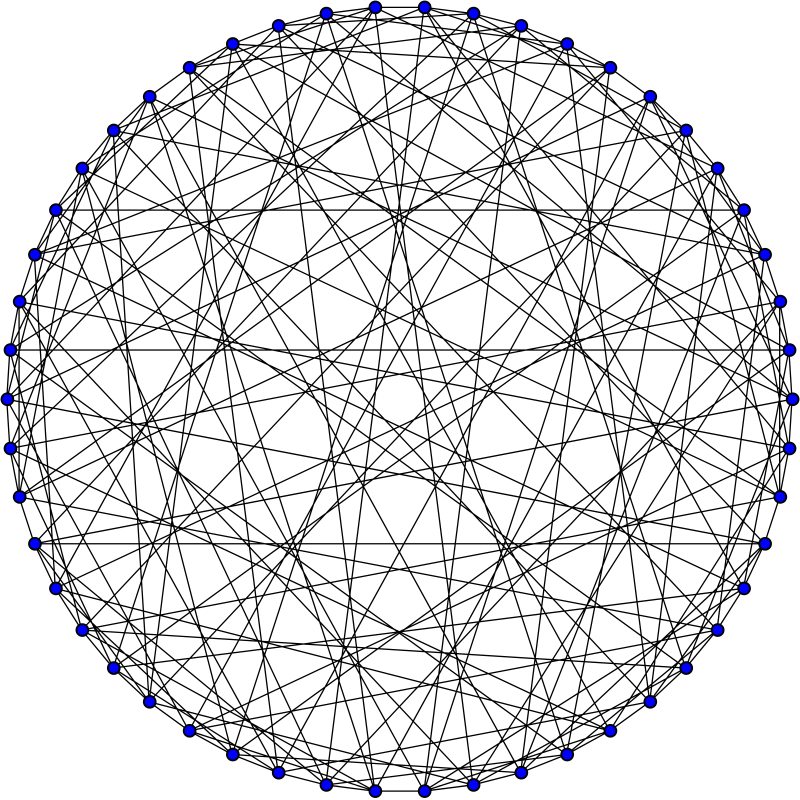
\includegraphics[scale=0.33]{Hoffman-Singleton_graph.png}
	\caption{Hoffman-singleton graph is Moore graph with $d=7$ and $k=2$ }
\end{figure}

%====================================================================================================================================================
% END OF INTRODUCTION TO DEGREE DIAMETER PROBLEM
%====================================================================================================================================================

%====================================================================================================================================================
% GRAPHS NON MOORE'S
%====================================================================================================================================================

\subsection{Graphs of order close to the Moore bound}
To facilitate the explanations, any graph of maximum degree $d$ and diameter $k$ will be called a $(d,k)$-{\em graph}. Because for $d\ge 3$ and $k\ge 2$ there are only a few $(d,k)$-graphs of order equal to the value $M_{d,k}$ of the Moore bound, researchers have tried to construct $(d,k)$-graphs of order as close to $M_{d,k}$ as possible. For a $(d,k)$-graph of order $M_{d,k}-\delta$ the quantity $\delta$ is knwn as the {\em defect}, and then we speak about a $(d,k,-\delta)$-graph; we note that this terminology is only used for `small' defects.
\medskip

There are a number of results concerning graphs with small defect. For example, Erd\"os, Fajtlowitcz and Hoffman proved \cite{Erd-Faj} that there is no graph of degree $d$ and diameter $2$ with $\delta = 1$ apart from the cycle of length $4$. In the case of $\delta = 2$ and $d = 2$ all the $(d,k,-2)$-graphs are the cycles of length $2k-1$. For $\delta-2$ and $d \geq 3$ only five graphs are known at present, namely, two $(3,2,-2)$-graphs of order $8$, one $(4,2,-2)$-graph of order $15$, one $(5,2,-2)$-graph of order $24$, and one $(3,3,-2)$-graph of order $20$; for details we refer to \cite{Mil-Sir}.

\subsection{Constructions of large graphs}
A different approach to finding $(d,k)$-graphs of order close to the Moore bound is by constructing appropriate `large' $(d,k)$-graphs. In most cases the constructions use combinatorics on words or algebraic structures such as groups and fields, so that the resulting graphs turn out to be rich in symmetries, or even vertex-transitive (and sometimes even Cayley).
\medskip

For a long time one of the asymptotically best families was the one of the \textit{undirected de Brujin graphs}, which are $(d,k)$ graphs for even $d$ and yield the lower bound
\begin{equation*}
	n_{d,k} \geq \left( \frac{d}{2} \right)^{k}.
\end{equation*}

This bound was improved by Baskoro and Miller \cite{Bas-Mil} to
\begin{equation}
	n_{d,k} \geq \left( \frac{d}{2} \right)^{k} +  \left( \frac{d}{2} \right)^{k-1}
\end{equation}	

In the special case of diameter $k=2$, modified Brown graphs can give for sufficiently large $d$ the bound
\begin{equation*}
	n_{d,2} \geq d^{2} - 2d^{1+\varepsilon}
\end{equation*}	
where the number $\varepsilon < 1$ depends on results about gaps between consecutive prime numbers; see \cite{Bev-Ers} for details about the current development.

\subsection{Graph lifting}
Graph lifting is a technique by which one may produce `large' graphs with certain required properties from suitable `small' graphs. The technique is well-known in topological and algebraic graph theory and for historical and mathematical details we refer to the monograph \cite{Gro-Tuc}. The technique can be described in the language of the so-called voltage assignments, which we briefly present next.
\medskip

Let $G$ be a graph. Although our graphs are undirected, we will preassign a direction to every edge. An edge with a preassigned direction is an {\em arc}. If $e$ is an arc of $G$, by the symbol $e^{-1}$ we denote the {\em reverse} of $e$, obtained simply by changing the preassigned direction on the edge. Let $D(G)$ be the set of all arcs of $G$; it follows that the size of $D(G)$ is twice the number of edges of $G$.
\medskip

Let $G$ be a graph as above and let $\Gamma$ be a finite group. The mapping
\begin{align*}
	\alpha: D(G) \rightarrow \Gamma
\end{align*}	
will be called a {\em voltage assignment} if $\alpha(e^{-1})$ = $(\alpha(e))^{-1}$, for any arc $e \in D(G)$.
\medskip

Out of the graph $G$ and the voltage assignment $\alpha$ as introduced above one can construct a `larger' graph, called the {\em lift} of $G$ (under the assignment $\alpha$) and denoted $G^{\alpha}$. The vertex set and the dart set of the new graph are defined as follows:
\begin{align*}
	V(G^{\alpha}) = V(G) \times \Gamma \\
	E(G^{\alpha}) = E(G) \times \Gamma
\end{align*}	
with the condition that if an arc $e$ emanates from a vertex $u$ and terminates in a vertex $v$ in the {\em base graph} $G$, then for every $g\in \Gamma$ there is a dart $(e,g)$ emanating from the vertex $(u,g)$ and terminating in the vertex $(v,g\alpha(e)$. It follows that right multiplication by $\alpha(e)$ permutes the terminal vertices of arcs $(e,g)$ emanating from the vertices $(u,g)$. At the same time this right multiplication induces a group of automorphisms of the lift acting freely on vertices and isomorphic to the {\em voltage group} $\Gamma$. Note that $G^{\alpha}$ can be considered to be an undirected graph, because the arcs $(e,g)$ and $(e^{-1},g\alpha(e))$ are reverse of each other.    \medskip

%% Example of Hoffman-Singleton lift.

This procedure can be reversed in the following sense, cf. \cite{Gro-Tuc}. Let $\tilde G$ be a graph and let $\Gamma$ be a group of automorphisms of $\tilde G$ that acts freely on vertices of $\tilde G$. Then $\tilde G$ is a lift of a `smaller' graph, denoted $\tilde G/\Gamma$ and called a {\em quotient}, which is obtained from $\tilde G$ by letting $\Gamma$-orbits of the vertex set and the arc set of $\tilde G$ to be vertices and arcs of the quotient, with incidence inherited from $\tilde G$.
\medskip

Of course, degrees of all the vertices $(u,g)$ in the lift are equal to the degree of $u$ in the base graph. An advantage of lifting is that the diameter of the lift can be conveniently controlled by properties of the base graph $G$ and the voltage assignment $\alpha$ as well. A {\em walk} of length $\ell$ in $G$ is any sequence  $W=e_1e_2\ldots e_{\ell}$ of consecutive arcs of $G$, and the voltage $\alpha(W)$ of the walk is simply the product $\alpha(W)=\alpha(e_1)\alpha(e_2)\cdots \alpha(e_{\ell})$. Then (cf. e.g. the survey \cite{Mil-Sir}), the lift $G^{\alpha}$ has diameter at most $k$ if for any two vertices $u,v$ of $G$ and for any element $g\in \Gamma$ there is a walk $W$ of length at most $k$ emanating from $u$ and terminating at $v$ such that $\alpha(W)=g$; in the case when $u=v$ we also require that $g\ne 1$.
\medskip

A number of the largest currently known ${d,k}$-graphs can be described as lifts. For example, all the graphs giving the values of $n_{3,7}$, $n_{3,8}$, $n_{4,4}$, $n_{5,3}$, $n_{5,5}$, $n_{6,3}$, $n_{6,4}$, $n_{7,3}$, $n_{14, 3}$ and $n_{16,2}$ obtained by computer search turn out to be lifts \cite{Mil-Sir}.



\subsection{Cayley graphs}
Let $\Gamma$ be a group and let $S\subset \Gamma$ be a symmetric unit-free generating set for $\Gamma$; that is, we require that $S=S^{-1}$ and $1\notin S$. The $\textit{Cayley graph}$ $C(\Gamma,S)$ is the graph with vertex set $\Gamma$ in which vertices $a,b$ are adjacent if $a^{-1}b\in S$. Observe that now the group $\Gamma$ acts regularly and hence freely on the vertex set of $C(\Gamma,S)$ as a group of automorphisms, so that the quotient graph $C(\Gamma,S)/\Gamma$ has just one vertex. By the remark in the previous section about groups of automorphisms acting freely in vertices it follows that Cayley graphs are simply lifts of one-vertex graphs (which will in general contain multiple loops and semi-edges but we will not go into the corresponding details).
\medskip

The diameter testing of lifts now easily translates into testing diameter of Cayley graphs as follows: A Cayley graph $C(\Gamma,S)$ has diameter at most $k$ if and only if every element of $\Gamma$ can be expressed as a product of at most $k$ elements of the generating set $S$. Equivalently, the diameter of a Cayley graph $C(\Gamma,S)$ is {\em equal} to $k$ if and only if $k$ is the smallest number such that every element of $\Gamma$ can be expressed as a product of at most $k$ elements of $S$.
\medskip

By $Cay_{d,k}$ we denote the largest order of a Cayley $(d,k)$-graph. In \cite{Jaj-Mac} it was proved that for every fixed $d \geq 3$ and $c \geq 2$ there is a set $A$ of natural numbers with positive density s.t. $C_{d,k} \leq M_{d,k}-c$ for all $k\in A$.
\medskip

The currently best available lower bound on $C_{d,2}$ was obtained by \v{S}iagiov\'a and \v{S}ir\'a\v{n} \cite{Sia-Sir} and reads as follows. Let $D = \{ 2^{2m+\mu}+(2+\delta)2^{m+1}-6,m \geq 1, \mu \in \{0,1\} \}$. Then, for every $d\in D$ one has $C_{d,2} > d^{2} - 6\sqrt{2}d^{3/2}$.

In the special case of Cayley graphs of diameter $k=2$ on Abelian groups there is a relatively straightforward lower bound of the form
\begin{equation*}
	n_{d,2} \geq \lfloor \frac{d+2}{2} \rfloor \lceil \frac{d + 2}{2} \rceil
\end{equation*}	
obtained by considering the product of cyclic groups $Z_{ \lfloor (d+2)/2  \rfloor) } \times Z_{ \lceil (d+2)/2 \rceil }$, with generating set consisting of all pairs $(x_1,x_2)$ with one of the entries equal to zero.

\subsection{General linear and special linear groups}

Linear groups are usually described in terms of linear transformations of vector spaces over general fields. For our purposes it will be sufficient to work with a more concrete description and restricted to finite fields. Let $q$ be a power of a prime and let $GF(q)$ be the Galois field of order $q$. The {\em general linear group} $GL(m,q)$ consists of all non-singular $m\times m$ matrices over $GF(q)$ under multiplication of matrices in the usual sense. By an elementary fact in group theory the order of $GL(m,q)$ is equal to $(q^m - 1)(q^m - q) \cdots (q^m - q^{n-1})$. The {\em special linear group} $SL(m,q)$ is the subgroup of $GL(m,q)$ consisting of matrices with determinant equal to $1$; its order is $|SL(m,q)| = |GL(m,q)|/(q-1)$.
\medskip

We will be particularly interested in the case $m=2$ and $q=p$ for some prime numbers $p$, and in Cayley graphs of diameter $2$ arising from the groups $SL(2,p)$. To the best of our knowledge such a study has not appeared in the available literature.

\newpage
\section{Results}

\subsection{Example of Cayley graph}

For example we generate Cayley graph on group $SL(2,3)$ with order $|SL(2,3)| = 24$ consiting of \\ \\
$
SL(2,3) = 
\bigg\{ 
\begin{bmatrix}
	1 & 0 \\
	0 & 1
\end{bmatrix},
\begin{bmatrix}
	0 & 1 \\
	2 & 0
\end{bmatrix},
\begin{bmatrix}
	0 & 1 \\
	2 & 1
\end{bmatrix},
\begin{bmatrix}
	0 & 1 \\
	2 & 2
\end{bmatrix},
\begin{bmatrix}
	0 & 2 \\
	1 & 0
\end{bmatrix},
\begin{bmatrix}
	0 & 2 \\
	1 & 1
\end{bmatrix},
\begin{bmatrix}
	0 & 2 \\
	1 & 2
\end{bmatrix},
\begin{bmatrix}
	1 & 0 \\
	1 & 1
\end{bmatrix},
\begin{bmatrix}
	1 & 0 \\
	2 & 1
\end{bmatrix},
\begin{bmatrix}
	1 & 1 \\
	0 & 1
\end{bmatrix}, \\
\begin{bmatrix}
	1 & 1 \\
	1 & 2
\end{bmatrix},
\begin{bmatrix}
	1 & 1 \\
	2 & 0
\end{bmatrix},
\begin{bmatrix}
	1 & 2 \\
	0 & 1
\end{bmatrix},
\begin{bmatrix}
	1 & 2 \\
	1 & 0
\end{bmatrix},
\begin{bmatrix}
	1 & 2 \\
	2 & 2
\end{bmatrix},
\begin{bmatrix}
	2 & 0 \\
	0 & 2
\end{bmatrix},
\begin{bmatrix}
	2 & 0 \\
	1 & 2
\end{bmatrix},
\begin{bmatrix}
	2 & 0 \\
	2 & 2
\end{bmatrix},
\begin{bmatrix}
	2 & 1 \\
	0 & 2
\end{bmatrix},
\begin{bmatrix}
	2 & 1 \\
	1 & 1
\end{bmatrix},
\begin{bmatrix}
	2 & 1 \\
	2 & 0
\end{bmatrix},
\begin{bmatrix}
	2 & 2 \\
	0 & 2
\end{bmatrix}, \\
\begin{bmatrix}
	2 & 2 \\
	1 & 0
\end{bmatrix},
\begin{bmatrix}
	2 & 2 \\
	2 & 1
\end{bmatrix} 
\bigg\}
$. \\ \\ 
For generating set $S$ with three pairs of elements and its inverses \\ \\ 
$
S = 
\bigg\{ 
\begin{bmatrix}
	1 & 1 \\
	1 & 2
\end{bmatrix},
\begin{bmatrix}
	2 & 2 \\
	2 & 1
\end{bmatrix},
\begin{bmatrix}
	2 & 2 \\
	0 & 2
\end{bmatrix},
\begin{bmatrix}
	2 & 1 \\
	0 & 2
\end{bmatrix},
\begin{bmatrix}
	0 & 2 \\
	1 & 1
\end{bmatrix},
\begin{bmatrix}
	1 & 1 \\
	2 & 0
\end{bmatrix}
\bigg\} 
$ \\ \\
Cayley graph $C(SL(2,3),S)$ has order 24, $d=6$ and $k=2$.  

\begin{figure}[!ht]
	\centering
	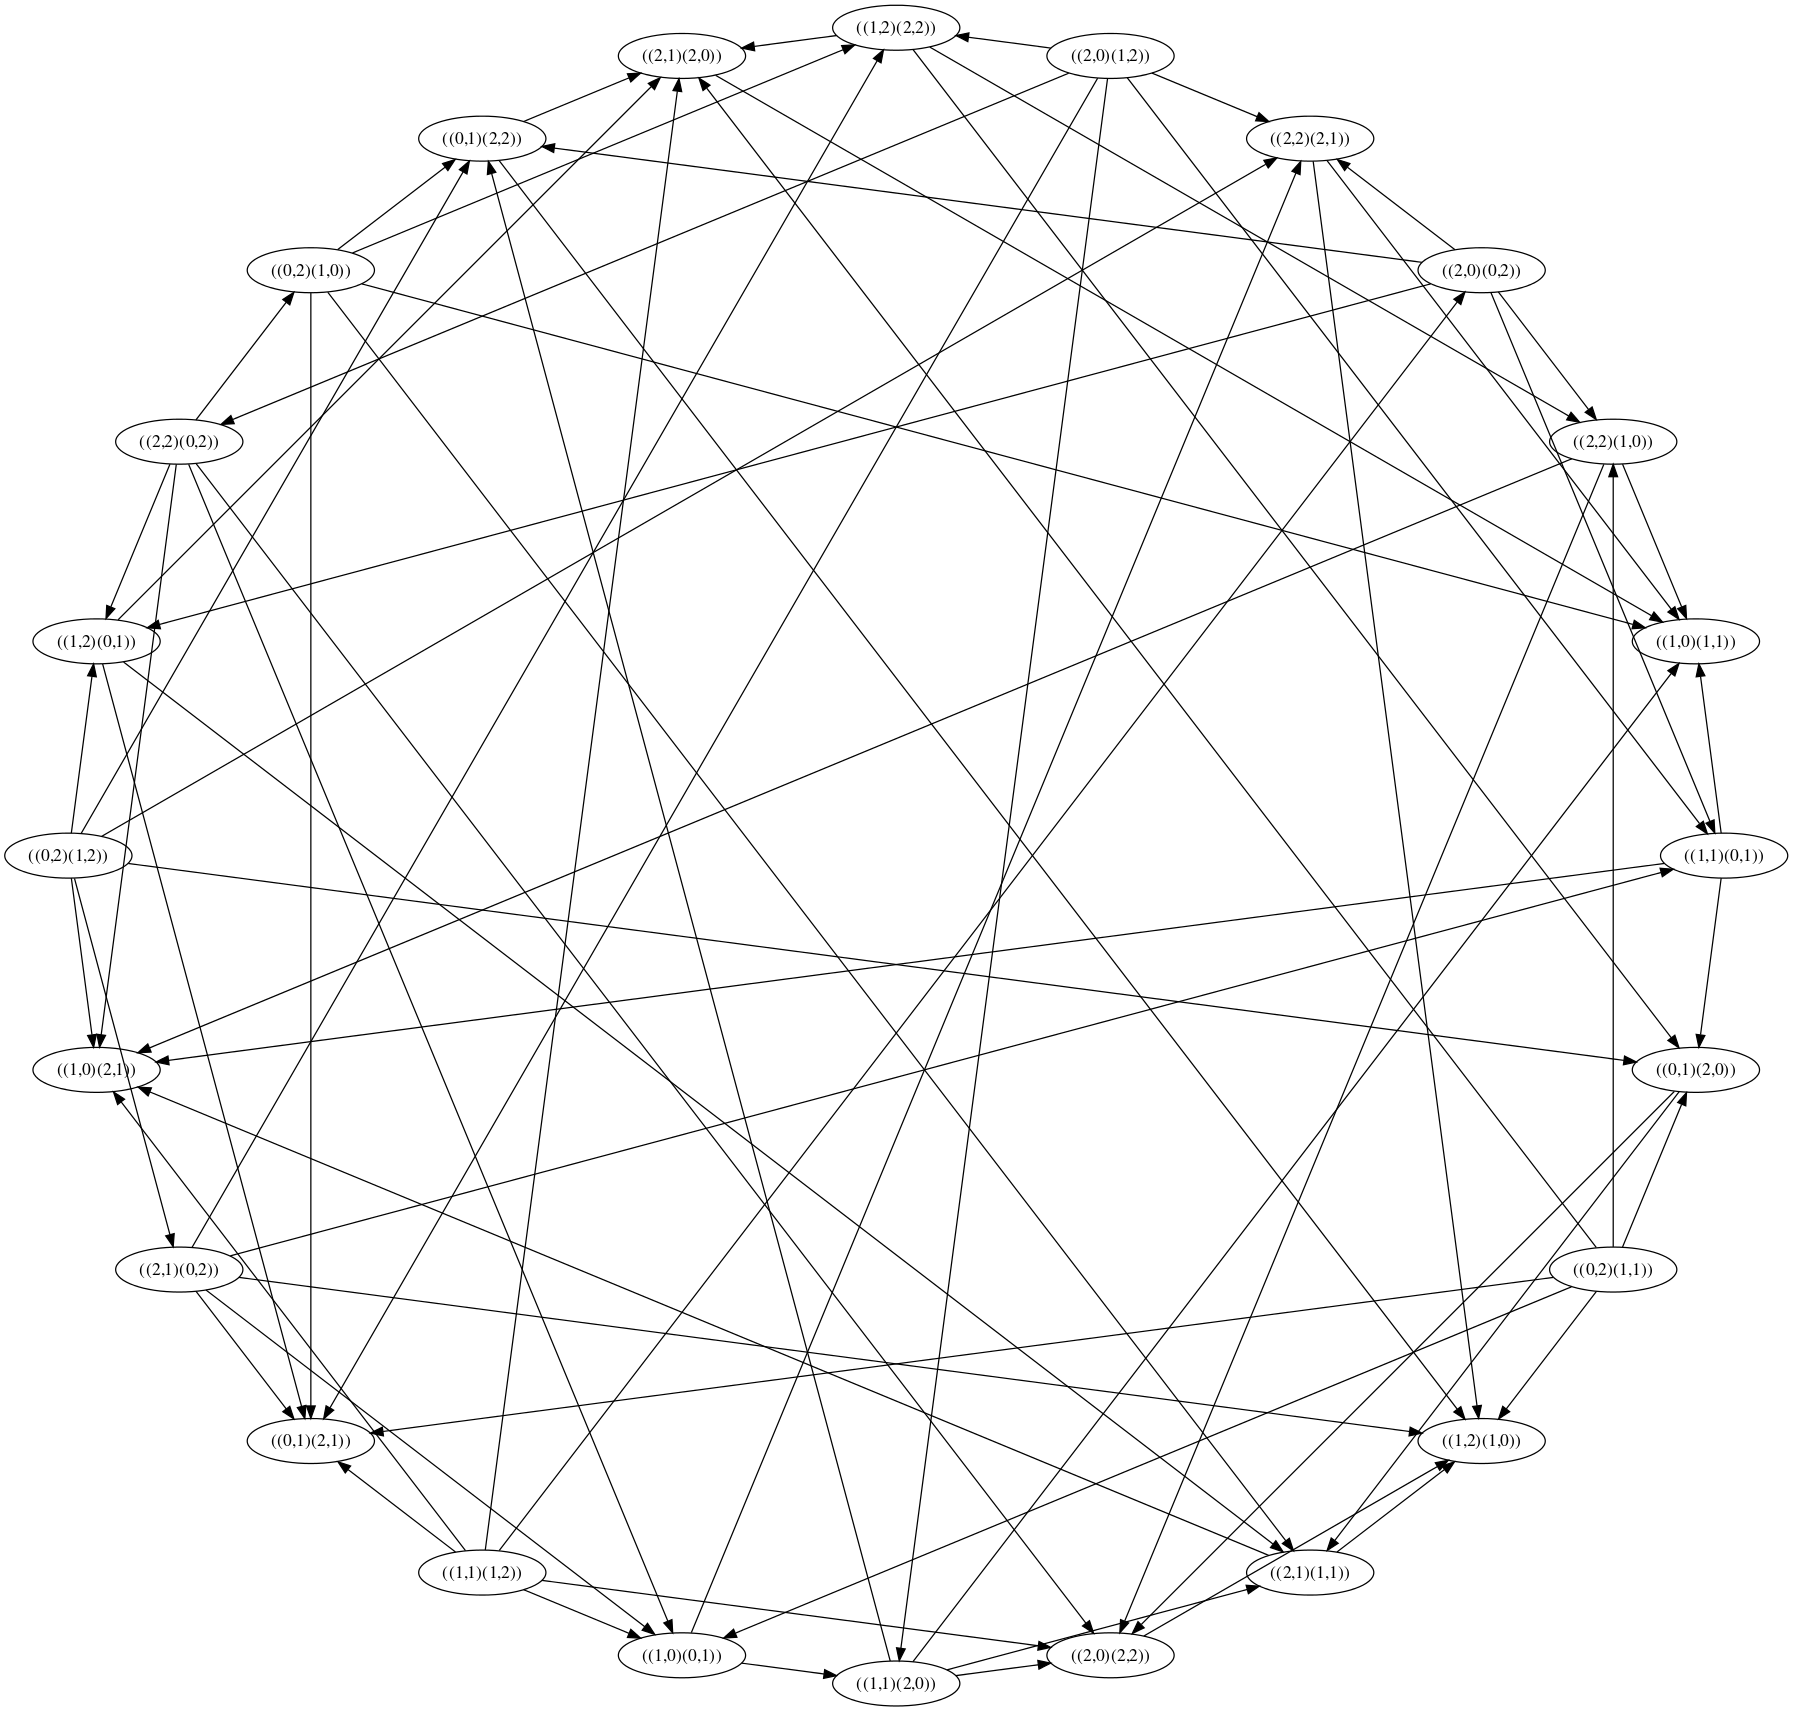
\includegraphics[scale=0.2]{example.png}
	\caption{ Output of circos ~\cite{Circos} of $C(SL(2,3), S)$ }
\end{figure}

The generating set S of the group $G=SL(2,3)$ in this example has the form $\{ x_1,x_1^{-1},x_2,x_2^{-1},x_3,x_3^{-1}\}$. To verify that the Cayley graph $C(G,S)$ has diameter $2$ one would have to show that the set $S$ together with the identity and with all products $x_i^{\pm 1}y_j^{\pm 1}$ gives the entire group $G$. Although this could be done by hand in this example, we deferred this task to a code that we designed for a more general purpose and which we list below.

\lstset{
	basicstyle=\footnotesize,
	tabsize=2
}
\lstinputlisting[language=Perl, frame=sinlge]{perl.pl}
\begin{algorithm}
        \caption{Cayley graph generation}
        \label{alg1}    
        \algsetup{indent=1em}
        \begin{algorithmic}[1]
                \REQUIRE $generation\_set[], n$
                \STATE $stack[] \leftarrow generation\_set[]$
                \STATE $stack\_element \leftarrow stack[0]$
                \WHILE{$stack[]$ \NOT empty}
                        \FORALL{$generating\_element \leftarrow generation\_set[]$}
                                \STATE $multiplication\_result \leftarrow (stack\_element * generating\_element)$ mod $n$
                                \STATE $multiplication\_results[stack\_element]$ append $multiplication\_result$
                                \STATE $stack[]$ append $multiplication\_result$
                        \ENDFOR
                        \STATE shift to the left $stack[]$
                        \STATE $stack\_element \leftarrow stack[0]$
                \ENDWHILE
                \RETURN $multiplication\_results$
        \end{algorithmic}
\end{algorithm}

\subsection{Computer search of graphs}

Here we present results of computer search of graphs in $SL(2,5)$ group. Order for $SL(2,5) = 120$ and it's assumed that Cayley graph will yield all elements of group. In search we were looking for graphs with diameter two. Moore bound for given parameter is $d=11$ therefore search was done on degree $12$ and up to 21. 

Generation sets were random and we generated and tested diameter two for 50000 graphs for all degrees. \\ \\

\begin{tabular}[htbp]{l*{10}{c}r}
	$d$	& $12$ & $13$ & $14$ & $15$ & $16$ & $17$ & $18$ & $19$ & $20$ & $21$ \\
\hline
	Found graphs & $0$ & $0$  & $0$ & $1$ & $107$ & $345$ & $2451$  & $4120$ & $11669$ & $14926$ \\
\end{tabular} \\ \\ 

Search for graphs in $SL(2,7)$ with order $336$ has failed to find any graph for $d=20$ up to $25$.

\begin{thebibliography}{xx}

\bibitem{Bas-Mil} E. T. Baskoro and M. Miller, On the construction of networks with minimum diameter,
Australian Computer Science Communications C 15 (1993) 739�743.

\bibitem{Bev-Ers} D. Bevan, G. Erskine and R. Lewis, Large circulant graphs of fized diameter and arbitrary degree, Ars Math. ontemp. 13 (2017), 275--29.

\bibitem{Erd-Faj} P. Erd{\H o}s, S. Fajtlowicz and A.J. Hoffman,
Maximum degree in graphs of diameter 2, Networks 10
(1980), 87--90.

\bibitem{Exo-Jaj} G. Exoo and R. Jajcay, Dynamic cage survey, Electr. J. Combin. 15 (2008), Dynamic Survey DS16.

\bibitem{Gro-Tuc} J. L. Gross and T. W. Tucker, Topological Graph Theory. Wiley, 1987 and Dover, 2001.

\bibitem{Hof-Sin} A. J. Hoffman and R. R. Singleton, On Moore graphs with diameter $2$ and $3$, IBM J. Res. Develop. 4 (1960), 497--504.

\bibitem{Jaj-Mac} R. Jajcay, M. Ma\v{c}aj and J. \v{S}ir\'a\v{n}, 

\bibitem{Mil-Sir} M. Miller and J. \v{S}ir\'a\v{n},  Moore graphs and beyond: A survey, 2nd Ed., Electr. J. Combin. 2013, Dynamic Survey DS15.

\bibitem{Sia-Sir} J. \v{S}iagiov\'a and J. \v{S}ir\'a\v{n}, Approaching the Moore bound for diameter two by Cayley graphs, J. Combin. Theory Ser. B 102 (2012) 470--473.

\bibitem{Circos} Circo, http://circos.ca

\end{thebibliography}

\end{document}

\subsubsection{Star product and compounding}

Star product and compounding are techniques for producing large graphs with given degree and diameter. \\

Star product of two graphs $H$ and $K$. Fix orientation of $H$ and let $E$ be set of oriented edges of $H$. For each dart $uv \in E$, let $\phi_{uv}$ be a bijection on the set $V(K)$. Vertex set of star product $H \star K$ is $V(H) \times V(K)$, and a vertex $(u,k)$ is joined to $(v,l)$ in new graph if and only if either $u = v$ and $kl$ is an edge of $K$, or if $uv \in E$ and $l = \phi_{uv}(k)$.

Compounding of two graphs $G$ and $H$ is made by taking $|V(H)|$ copies of $G$, indexed by vertices of $H$, and joining of two copies $G_{u}$, $G_{v}$ of $G$ by edge whenever $uv$ is an edge of $H$.
